\section{必ずしも共鳴条件を満たさない場合}\label{nonreso_sec}
これまではシンプルにスピン干渉という現象を見るために、共鳴条件(\ref{pi2flipper_resonance})が満たされる場合のみを扱ってきた。しかし、実際の解析では共鳴条件を満たさない場合も扱う必要があるため、この章ではより一般的に必ずしも共鳴条件を満たさない場合に何が起こるかを見てゆく。


\subsection{スピンフリッパーの機能}
スピン干渉について考える前に、共鳴条件を満たさない場合のスピンフリッパーの機能について考えよう。

\paragraph{舞台とあらすじ}
一様磁場中に理想化されたRFスピンフリッパーがひとつ置かれた状況を考える。系は3つの領域I,II,IIIからなり、全体に$z$方向一様磁場$B_z$が、領域IIに$x$方向振動磁場$2B_r \cos \omega_s t$がかけられている。
\begin{figure}[h]
\centering
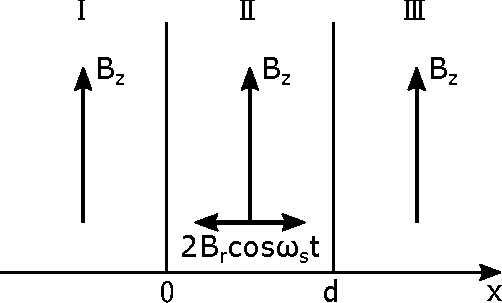
\includegraphics[height=3cm]{nonreso/resonance_setting1.pdf}
\end{figure}

これから述べるように、スピン上向きの中性子が領域Iから速度$v$で入射し領域IIを通って領域IIIに抜けるとき、領域IIIにおけるスピン上向き中性子の存在確率は
\begin{equation}
|\psi_{\mathrm{III}}^+|^2=\cos^2 \frac{\omega_A}{v}d+\left(\frac{\epsilon}{\omega_A}\right)^2\sin^2\frac{\omega_A}{v}d \label{Nonreso_flip}
\end{equation}
となる。ここで$\epsilon=\omega_s/2-\omega_z,\omega_A=\sqrt{\epsilon^2+\omega_r^2}$であり、$\omega_z=|\mu_n|B_z,\omega_r=|\mu_n|B_r$、$\mu_n$は中性子の磁気モーメント、$d$は領域IIの幅である。ここで定義した
\begin{equation}
\epsilon=\frac{\omega_s}{2}-\omega_z
\end{equation}
という量は共鳴からのずれを表す指標であり、この章で非常に重要な役割を演じる。

\begin{comment}
式(\ref{Nonreso_flip})を見ると$\epsilon=0$がなりたてば、$\omega_rd/v=\pi/2$を満たす速度の中性子に対して、領域IIIにおけるスピン上向き粒子の存在確率が0、すなわちスピン反転率が1になることがわかる。逆に$\epsilon \neq 0$のときはどのような速度の中性子に対しても反転率は1となり得ない。このように、$\epsilon=0$を満たす周波数の振動磁場をかけたときに限りスピンフリッパーを通り抜けた中性子のスピンが完全に反転し得る。これをスピンフリッパーの共鳴と呼び、$\epsilon=0$を共鳴条件と呼んだのであった。
\end{comment}

\renewcommand{\arraystretch}{1.5}

\paragraph{入射波}
スピンの量子化軸を$z$軸に選ぶと、領域IにおけるShr$\ddot{\mathrm{o}}$dinger方程式は%なぜか\''{o}が使えない
\begin{equation}
i\frac{\del \psi_\mathrm{I}}{\del t}= \Biggl[-\frac{1}{2m} \frac{\del^2}{\del x^2} \underbrace{-\mu_nB_z}_{+|\mu_n|Bz =\omega_z} \sigma_z\Biggr] \psi_\mathrm{I}
\end{equation}
入射中性子のスピンは上向きとしたので、そのエネルギーを$\omega_0$とすると、領域Iにおける波動関数の入射成分はスピン上下の2成分表示で
\begin{equation}
\psi_\mathrm{I}^{\mathrm{in}}=\begin{pmatrix} 1\\0 \end{pmatrix} \e^{i k_0^+ x -i\omega_0 t}
\end{equation}
と書ける。ここで$k_0^+=\sqrt{2m(\omega_0 -\omega_z)}$。
\renewcommand{\arraystretch}{1}

\paragraph{領域II}
領域IIにおける磁場を
\begin{equation}
\bm{B}_{\mathrm{II}}=\hat{\bm{x}} (2B_r)\cos \omega_s t+\hat{\bm{z}} B_z
\end{equation}
と書く。ただし$\hat{\bm{x}},\hat{\bm{z}}$はそれぞれx,z軸正の向きの単位ベクトル。$|B_r| \ll |B_z|$のときには、\ref{pi2flipper_sec}章で述べた理由により振動磁場を次のような$xy$平面上の回転磁場に置き換えてよい:
\begin{equation}
\hat{\bm{x}} (2B_r)\cos \omega_s t \rightarrow \hat{\bm{x}} B_r \cos \omega_s t+\hat{\bm{y}} \sin \omega_s t
\end{equation}
したがって$|B_r| \ll |B_z|$のとき領域IIにおける磁場は
\begin{equation}
\bm{B}_{\mathrm{II}}\simeq \hat{\bm{x}} B_r\cos \omega_s t+\hat{\bm{y}} B_r \sin \omega_s t+\hat{\bm{z}} B_z
\end{equation}
となる。このとき領域IIにおけるShr$\ddot{\mathrm{o}}$dinger方程式は
\begin{align}
i\frac{\del \psi_{\mathrm{II}}}{\del t} &=\left[-\frac{1}{2m} \frac{\del^2}{\del x^2} -\bm{\mu}_n\cdot\bm{B}_\mathrm{II}\right] \psi_\mathrm{II}\notag \\
&=\left[-\frac{1}{2m} \frac{\del^2}{\del x^2} + |\mu_n| (\sigma_x B_r \cos\omega_s t+\sigma_y B_r\sin\omega_s t+\sigma_zB_z)\right] \psi_\mathrm{II} \notag \\
&=\left[-\frac{1}{2m} \frac{\del^2}{\del x^2} +\begin{pmatrix} \omega_z &\omega_r \e^{-i\omega_s t} \\\omega_r \e^{i\omega_s t} &-\omega_z \end{pmatrix}\right] \psi_\mathrm{II}
\end{align}
となる。まずハミルトニアンの時間依存性を除くために、$z$軸まわりの角速度$-\omega_s$の回転を表すユニタリ変換
\begin{equation}
U_T=\exp\left[+iS_z\omega_s t\right] =\exp\left[i\sigma_z\frac{\omega_s t}{2}\right]=\begin{pmatrix} \e^{i\omega_st/2} &0\\0&\e^{-i\omega_st/2}\end{pmatrix}
\end{equation}
を用いて
\begin{equation}
U_T \begin{pmatrix} \omega_z &\omega_r \e^{-i\omega_s t} \\\omega_r \e^{i\omega_s t} &-\omega_z \end{pmatrix} U_T^\dagger =\begin{pmatrix} \omega_z &\omega_r\\ \omega_r&-\omega_z \end{pmatrix}
\end{equation}
がなりたつことに注意すると、
\begin{equation}
i\frac{\del}{\del t}(U_T \psi_\mathrm{II}) =\left[-\frac{1}{2m} \frac{\del^2}{\del x^2} +\begin{pmatrix} -(\frac{\omega_s}{2}-\omega_z) &\omega_r\\ \omega_r &\frac{\omega_s}{2}-\omega_z \end{pmatrix}\right] (U_T \psi_\mathrm{II})
\end{equation}
を得る。さらにこのハミルトニアンを対角的にするために
\begin{equation}
\begin{pmatrix} -(\frac{\omega_s}{2}-\omega_z) &\omega_r\\ \omega_r &\frac{\omega_s}{2}-\omega_z \end{pmatrix}=\omega_A\begin{pmatrix} \cos \theta&\sin \theta\\ \sin \theta &-\cos \theta \end{pmatrix}
\end{equation}
と書く。ここで$\epsilon=\omega_s/2-\omega_z,\omega_A=\sqrt{\epsilon^2+\omega_r^2}$として
\begin{equation}
\cos \theta=\frac{-\epsilon}{\omega_A} , \quad \sin \theta=\frac{\omega_r}{\omega_A}
\end{equation}
である。$y$軸まわりの角度$-\theta$回転を表すユニタリ変換
\begin{equation}
U_D=\exp\left[+iS_y \theta\right] =\exp\left[i\sigma_y \frac{\theta}{2}\right] =\begin{pmatrix} \cos\frac{\theta}{2}& \sin\frac{\theta}{2}\\  -\sin\frac{\theta}{2}& \cos\frac{\theta}{2}\end{pmatrix}
\end{equation}
を用いて
\begin{equation}
U_D \begin{pmatrix} \cos \theta&\sin \theta\\ \sin \theta &-\cos \theta \end{pmatrix} U_D^\dagger =\begin{pmatrix} 1&0\\0&-1\end{pmatrix}
\end{equation}
がなりたつことに注意すると、
\begin{equation}
i\frac{\del}{\del t}(U_DU_T \psi_\mathrm{II}) =\left[-\frac{1}{2m} \frac{\del^2}{\del x^2} +\omega_A \sigma_Z \right] (U_DU_T \psi_\mathrm{II})
\end{equation}
を得る。

\renewcommand{\arraystretch}{1.5}
したがって、領域IIにおける中性子のエネルギーを$\omega_n$とすると、定数$A_n^\pm,B_n^\pm$を用いて
\begin{equation}
\psi_D \equiv U_D U_T \psi_\mathrm{II} =\begin{pmatrix} A_n^+ \e^{ik_n^+x}+B_n^+\e^{-ik_n^+x} \\ A_n^- \e^{ik_n^-x}+B_n^-\e^{-ik_n^-x} \end{pmatrix} \e^{-i\omega_n t}
\end{equation}
と書けるから、領域IIにおける波動関数は
\begin{align}
\psi_\mathrm{II}&=U_T^\dagger U_D^\dagger \psi_D \notag \\
&=\begin{pmatrix} \e^{-i\omega_st/2} &0\\0&\e^{+i\omega_st/2}\end{pmatrix} \begin{pmatrix} \cos\frac{\theta}{2}& -\sin\frac{\theta}{2}\\  \sin\frac{\theta}{2}& \cos\frac{\theta}{2}\end{pmatrix} \begin{pmatrix} A_n^+ \e^{ik_n^+x}+B_n^+\e^{-ik_n^+x} \\ A_n^- \e^{ik_n^-x}+B_n^-\e^{-ik_n^-x} \end{pmatrix} \e^{-i\omega_n t} \notag \\
&=\begin{pmatrix} \left(A_n^+ \cos \frac{\theta}{2} \e^{ik_n^+x}+ B_n^+ \cos \frac{\theta}{2} \e^{-ik_n^+x} - A_n^- \sin \frac{\theta}{2} \e^{ik_n^-x}- B_n^- \sin \frac{\theta}{2} \e^{-ik_n^-x}\right) \e^{-i(\omega_n+\omega_s/2)t} \\ \left(A_n^+ \sin \frac{\theta}{2} \e^{ik_n^+x}+ B_n^+ \sin \frac{\theta}{2} \e^{-ik_n^+x} + A_n^- \cos \frac{\theta}{2} \e^{ik_n^-x}+ B_n^- \cos \frac{\theta}{2} \e^{-ik_n^-x}\right) \e^{-i(\omega_n-\omega_s/2)t} \end{pmatrix} \label{Nonreso_psi2}
\end{align}
と書ける。ここで$k_n^\pm=\sqrt{2m(\omega_n \mp \omega_A)}$。

\paragraph{領域IとIIの接続}
入射波$\psi_\mathrm{I}^\mathrm{in}$と$\psi_\mathrm{II}$が任意の時刻$t$で領域IとIIの境界($x=0$)において接続するためには
\begin{equation}
\omega_n=\omega_1 \equiv \omega_0 -\frac{\omega_s}{2}
\end{equation}
が必要である。そのとき
\begin{equation}
\psi_\mathrm{II}=\begin{pmatrix} \left(A_1^+ \cos \frac{\theta}{2} \e^{ik_1^+x}+ B_1^+ \cos \frac{\theta}{2} \e^{-ik_1^+x} - A_1^- \sin \frac{\theta}{2} \e^{ik_1^-x}- B_1^- \sin \frac{\theta}{2} \e^{-ik_1^-x}\right) \e^{-i\omega_0t} \\ \left(A_1^+ \sin \frac{\theta}{2} \e^{ik_1^+x}+ B_1^+ \sin \frac{\theta}{2} \e^{-ik_1^+x} + A_1^- \cos \frac{\theta}{2} \e^{ik_1^-x}+ B_1^- \cos \frac{\theta}{2} \e^{-ik_1^-x}\right) \e^{-i(\omega_0-\omega_s)t} \end{pmatrix}
\end{equation}
ここで$k_1^\pm=\sqrt{2m(\omega_0-\omega_s/2 \mp \omega_A)}$。

またこのことから、領域Iでの反射波を含めた全波動関数$\psi_\mathrm{I}$は
\begin{equation}
\psi_\mathrm{I} =I_0^+ \psi_\mathrm{I}^\mathrm{in} +\begin{pmatrix} R_0^+ \e^{-ik_0^+x}\e^{ -i\omega_0 t} \\ R_2^- \e^{-ik_2^-x}\e^{ -i (\omega_0-\omega_s)t} \end{pmatrix} =\begin{pmatrix} (I_0^+ \e^{ik_0^+x} +R_0^+\e^{-ik_0^+x} )\e^{-i\omega_0 t} \\ R_2^- \e^{-ik_2^-x}\e^{ -i (\omega_0-\omega_s)t} \end{pmatrix}
\end{equation}
と書ける。ここで$I_0^+,R_0^+,R_2^-$は定数であり、$k_0^+ =\sqrt{2m(\omega_0 -\omega_z)},k_2^- =\sqrt{2m(\omega_0 -\omega_s +\omega_z)}$である。

さて、ここで領域IとIIの接続を考えると、次の4つの式がなりたつ:
\begin{align}
\left\{\begin{array}{l}
A_1^+ \cos \frac{\theta}{2} +B_1^+\cos \frac{\theta}{2} -A_1^-\sin\frac{\theta}{2} -B_1^-\sin\frac{\theta}{2} = I_0^+ +R_0^+ \\
k_1^+(A_1^+ \cos \frac{\theta}{2} -B_1^+\cos \frac{\theta}{2} )-k_1^-(A_1^-\sin\frac{\theta}{2} -B_1^-\sin\frac{\theta}{2} )=k_0^+(I_0^--R_0^+)\\
A_1^+ \sin \frac{\theta}{2} +B_1^+\sin \frac{\theta}{2} +A_1^-\cos\frac{\theta}{2} +B_1^-\cos\frac{\theta}{2} = R_2^- \\
k_1^+(A_1^+ \sin \frac{\theta}{2} -B_1^+\sin \frac{\theta}{2}) +k_1^-(A_1^-\cos\frac{\theta}{2} -B_1^-\cos\frac{\theta}{2}) = -k_2^-R_2^-
\end{array} \right. \label{Nonreso_setsuzoku}
\end{align}

\paragraph{近似}
いま中性子の入射エネルギー$\omega_0$は、$\omega_z$や$\omega_s,\omega_r$などと比べて十分大きいとする。このとき
\begin{align}
&k_0^+ =\sqrt{2m(\omega_0 -\omega_z)} \simeq k_0 -\frac{\omega_z}{v} \label{Nonreso_k0+} \\
&k_1^{\pm} = \sqrt{2m(\omega_0-\omega_s/2 \mp \omega_A)} \simeq k_0 -\frac{\omega_s}{2v} \mp \frac{\omega_A}{v} \label{Nonreso_k1+-} \\
&k_2^- =\sqrt{2m(\omega_0 -\omega_s +\omega_z)} \simeq k_0 -\frac{\omega_s}{v} +\frac{\omega_z}{v}\label{Nonreso_k2-}
\end{align}
となる。ここで$k_0 \equiv \sqrt{2m\omega_0}$とした。さらに式(\ref{Nonreso_setsuzoku})のように両辺で$k_0$が打ち消し合わないときは
\begin{equation}
k_n^\pm \simeq k_0\label{Nonreso_kn+-}
\end{equation}
と近似する。後で見るようにこれは反射波を無視することと同値である。

この近似の下で式(\ref{Nonreso_setsuzoku})は次のように変形される:
\begin{align}
&\left\{\begin{array}{l}
A_1^+ \cos \frac{\theta}{2} +B_1^+\cos \frac{\theta}{2} -A_1^-\sin\frac{\theta}{2} -B_1^-\sin\frac{\theta}{2} = I_0^+ +R_0^+ \\
k_0(A_1^+ \cos \frac{\theta}{2} -B_1^+\cos \frac{\theta}{2} )-k_0(A_1^-\sin\frac{\theta}{2} -B_1^-\sin\frac{\theta}{2} )=k_0(I_0^--R_0^+)\\
A_1^+ \sin \frac{\theta}{2} +B_1^+\sin \frac{\theta}{2} +A_1^-\cos\frac{\theta}{2} +B_1^-\cos\frac{\theta}{2} = R_2^- \\
k_0(A_1^+ \sin \frac{\theta}{2} -B_1^+\sin \frac{\theta}{2}) +k_0(A_1^-\cos\frac{\theta}{2} -B_1^-\cos\frac{\theta}{2}) = -k_0R_2^-
\end{array} \right.  \notag \\
&\Rightarrow \left\{\begin{array}{l}
A_1^+ \cos \frac{\theta}{2} +B_1^+\cos \frac{\theta}{2} -A_1^-\sin\frac{\theta}{2} -B_1^-\sin\frac{\theta}{2} = I_0^+ +R_0^+ \\
A_1^+ \cos \frac{\theta}{2} -B_1^+\cos \frac{\theta}{2} -A_1^-\sin\frac{\theta}{2} -B_1^-\sin\frac{\theta}{2} =I_0^--R_0^+\\
A_1^+ \sin \frac{\theta}{2} +B_1^+\sin \frac{\theta}{2} +A_1^-\cos\frac{\theta}{2} +B_1^-\cos\frac{\theta}{2} = R_2^- \\
A_1^+ \sin \frac{\theta}{2} -B_1^+\sin \frac{\theta}{2} +A_1^-\cos\frac{\theta}{2} -B_1^-\cos\frac{\theta}{2} = -R_2^-
\end{array} \right.  \notag \\
&\Rightarrow \left\{\begin{array}{l}
A_1^+ \cos \frac{\theta}{2} -A_1^-\sin\frac{\theta}{2}= I_0^+ \\
B_1^+\cos \frac{\theta}{2} -B_1^-\sin\frac{\theta}{2} =R_0^+\\
A_1^+ \sin \frac{\theta}{2}+A_1^-\cos\frac{\theta}{2}= 0 \\
B_1^+\sin \frac{\theta}{2} -B_1^-\cos\frac{\theta}{2} = R_2^-
\end{array} \right.  \notag \\
&\Rightarrow \left\{\begin{array}{l}
A_1^+ = I_0^+\cos\frac{\theta}{2} \\
A_1^- =-I_0^+\sin\frac{\theta}{2} \\
B_1^+=R_0^+\cos\frac{\theta}{2}+R_2^-\sin\frac{\theta}{2} \\
B_1^-=R_2^-\cos\frac{\theta}{2}-R_0\sin\frac{\theta}{2}
\end{array} \right. \label{Nonreso_1and2}
\end{align}

\paragraph{領域III}
領域IIIにおけるShr$\ddot{\mathrm{o}}$dinger方程式は領域Iと同じで
\begin{equation}
i\frac{\del \psi_\mathrm{III}}{\del t}= \left[-\frac{1}{2m} \frac{\del^2}{\del x^2} +\omega_z \sigma_z\right] \psi_\mathrm{III}
\end{equation}
である。$\psi_\mathrm{II}$と$\psi_\mathrm{III}$が任意の時刻$t$で領域IIとIIIの境界($x=d$)において接続するためには、式(\ref{Nonreso_psi2})より、領域IIIにおける中性子のエネルギーがスピン上向きに対しては$\omega_0$、スピン下向きに対しては$\omega_0-\omega_s$であることが必要である。よって領域IIIにおける波動関数$\psi_\mathrm{III}$は定数$C_0^+,C_2^-$を用いて
\begin{equation}
\psi_\mathrm{III}=\begin{pmatrix} C_0^+ \e^{ik_0^+ x}\e^{-i\omega_0 t} \\ C_2^- \e^{ik_2^- x}\e^{-i(\omega_0-\omega_s) t} \end{pmatrix}
\end{equation}
と書ける。ここで$k_0^+=\sqrt{2m(\omega_0-\omega_z)},k_2^-=\sqrt{2m(\omega_0-\omega_s+\omega_z)}$。

\paragraph{領域IIとIIIの接続}
次に領域IIとIIIの接続を考える。前述の通り、波数の内、両辺で$k_0$が打ち消しあいその差が現れるもの(指数の肩に乗っているもの)については式(\ref{Nonreso_k0+}),(\ref{Nonreso_k1+-}),(\ref{Nonreso_k2-})のように、両辺で$k_0$が打ち消し合わないもの(指数の肩から降りているもの)については式(\ref{Nonreso_kn+-})のように近似する。すると次の4つの式がなりたつ:
\begin{align}
&\left\{\begin{array}{l}
\left(A_1^+ \cos \frac{\theta}{2} \e^{-i\frac{\omega_A}{v}d}+B_1^+\cos \frac{\theta}{2} \e^{i\frac{\omega_A}{v}d}-A_1^-\sin\frac{\theta}{2}\e^{i\frac{\omega_A}{v}d} -B_1^-\sin\frac{\theta}{2}\e^{-i\frac{\omega_A}{v}d} \right)\e^{i(k_0-\frac{\omega_s}{2v})d}= C_0^+\e^{i(k_0-\frac{\omega_z}{v})d} \\
\left(A_1^+ \cos \frac{\theta}{2} \e^{-i\frac{\omega_A}{v}d}-B_1^+\cos \frac{\theta}{2} \e^{i\frac{\omega_A}{v}d}-A_1^-\sin\frac{\theta}{2}\e^{i\frac{\omega_A}{v}d} +B_1^-\sin\frac{\theta}{2}\e^{-i\frac{\omega_A}{v}d} \right)\e^{i(k_0-\frac{\omega_s}{2v})d}= C_0^+\e^{i(k_0-\frac{\omega_z}{v})d} \\
\left(A_1^+ \sin \frac{\theta}{2} \e^{-i\frac{\omega_A}{v}d}+B_1^+\sin \frac{\theta}{2} \e^{i\frac{\omega_A}{v}d}+A_1^-\cos\frac{\theta}{2}\e^{i\frac{\omega_A}{v}d} +B_1^-\cos\frac{\theta}{2}\e^{-i\frac{\omega_A}{v}d} \right)\e^{i(k_0-\frac{\omega_s}{2v})d}= C_2^-\e^{i(k_0-\frac{\omega_s}{v}+\frac{\omega_z}{v})d} \\
\left(A_1^+ \sin \frac{\theta}{2} \e^{-i\frac{\omega_A}{v}d}-B_1^+\sin \frac{\theta}{2} \e^{i\frac{\omega_A}{v}d}+A_1^-\cos\frac{\theta}{2}\e^{i\frac{\omega_A}{v}d} -B_1^-\cos\frac{\theta}{2}\e^{-i\frac{\omega_A}{v}d} \right)\e^{i(k_0-\frac{\omega_s}{2v})d}= C_2^-\e^{i(k_0-\frac{\omega_s}{v}+\frac{\omega_z}{v})d} \\
\end{array} \right.  \notag \\
&\Rightarrow \left\{\begin{array}{l}
\left(A_1^+ \cos \frac{\theta}{2} \e^{-i\frac{\omega_A}{v}d}+B_1^+\cos \frac{\theta}{2} \e^{i\frac{\omega_A}{v}d}-A_1^-\sin\frac{\theta}{2}\e^{i\frac{\omega_A}{v}d} -B_1^-\sin\frac{\theta}{2}\e^{-i\frac{\omega_A}{v}d} \right)\e^{-i\frac{\frac{\omega_s}{2}-\omega_z}{v}d}= C_0^+\\
\left(A_1^+ \cos \frac{\theta}{2} \e^{-i\frac{\omega_A}{v}d}-B_1^+\cos \frac{\theta}{2} \e^{i\frac{\omega_A}{v}d}-A_1^-\sin\frac{\theta}{2}\e^{i\frac{\omega_A}{v}d} +B_1^-\sin\frac{\theta}{2}\e^{-i\frac{\omega_A}{v}d} \right)\e^{-i\frac{\frac{\omega_s}{2}-\omega_z}{v}d}= C_0^+\\
\left(A_1^+ \sin \frac{\theta}{2} \e^{-i\frac{\omega_A}{v}d}+B_1^+\sin \frac{\theta}{2} \e^{i\frac{\omega_A}{v}d}+A_1^-\cos\frac{\theta}{2}\e^{i\frac{\omega_A}{v}d} +B_1^-\cos\frac{\theta}{2}\e^{-i\frac{\omega_A}{v}d} \right)\e^{i\frac{\frac{\omega_s}{2}-\omega_z}{v}d}= C_2^-\\
\left(A_1^+ \sin \frac{\theta}{2} \e^{-i\frac{\omega_A}{v}d}-B_1^+\sin \frac{\theta}{2} \e^{i\frac{\omega_A}{v}d}+A_1^-\cos\frac{\theta}{2}\e^{i\frac{\omega_A}{v}d} -B_1^-\cos\frac{\theta}{2}\e^{-i\frac{\omega_A}{v}d} \right)\e^{i\frac{\frac{\omega_s}{2}-\omega_z}{v}d}= C_2^- \\
\end{array} \right.  \notag \\
&\Rightarrow \left\{\begin{array}{l}
\left(A_1^+ \cos \frac{\theta}{2} \e^{-i\frac{\omega_A}{v}d}-A_1^-\sin\frac{\theta}{2}\e^{i\frac{\omega_A}{v}d} \right)\e^{-i\frac{\epsilon}{v} d}= C_0^+\\
\left(B_1^+\cos \frac{\theta}{2} \e^{i\frac{\omega_A}{v}d}-B_1^-\sin\frac{\theta}{2}\e^{-i\frac{\omega_A}{v}d} \right)\e^{-i\frac{\epsilon}{v} d}= 0\\
\left(A_1^+ \sin \frac{\theta}{2} \e^{-i\frac{\omega_A}{v}d}+A_1^-\cos\frac{\theta}{2}\e^{i\frac{\omega_A}{v}d} \right)\e^{i\frac{\epsilon}{v} d}= C_2^- \\
\left(B_1^+\sin \frac{\theta}{2} \e^{i\frac{\omega_A}{v}d}+B_1^-\cos\frac{\theta}{2}\e^{-i\frac{\omega_A}{v}d} \right)\e^{i\frac{\epsilon}{v} d}= 0
\end{array} \right. \notag \\
&\Rightarrow \left\{\begin{array}{l}
C_0^+=\left(A_1^+ \cos \frac{\theta}{2} \e^{-i\frac{\omega_A}{v}d}-A_1^-\sin\frac{\theta}{2}\e^{i\frac{\omega_A}{v}d} \right)\e^{-i\frac{\epsilon}{v} d}\\
C_2^-=\left(A_1^+ \sin \frac{\theta}{2} \e^{-i\frac{\omega_A}{v}d}+A_1^-\cos\frac{\theta}{2}\e^{i\frac{\omega_A}{v}d} \right)\e^{i\frac{\epsilon}{v} d}\\
B_1^+=0\\
B_1^-= 0
\end{array} \right. \label{Nonreso_2and3}
\end{align}
%ここで$\epsilon=\omega_s/2-\omega_z$とした。
%\end{comment}


\paragraph{結末}
したがって式(\ref{Nonreso_1and2}),(\ref{Nonreso_2and3})より
\begin{equation}
\left\{ \begin{array}{l}
A_1^+=I_0^+ \cos \frac{\theta}{2} \\
A_1^-=-I_0^+ \cos \frac{\theta}{2} \\
B_1^+=0 \\
B_1^-=0 \\
C_0^+=I_0^+\left(\sin^2 \frac{\theta}{2} \e^{i\frac{\omega_A}{v}d} +\cos^2 \frac{\theta}{2} \e^{-i\frac{\omega_A}{v}d} \right)  \e^{-i\frac{\epsilon}{v}d} \\
C_2^-=I_0^+ \sin\frac{\theta}{2}\cos\frac{\theta}{2} \left(\e^{-i\frac{\omega_A}{v}d}-\e^{i\frac{\omega_A}{v}d}\right) \e^{i\frac{\epsilon}{v}d}\\
R_0^+=0\\
R_2^-=0
\end{array} \right.
\end{equation}
を得る。前述の通り$B_1^\pm=R_0^+=R_2^-=0$、すなわち全ての境界における反射波はゼロとなる。いま$|\psi_\mathrm{I}|^2=|I_0^+|^2=1$と規格化すると、$I_0^+=1$ととってよい。そのとき

%\renewcommand{\arraystretch}{1}
\begin{align}
\psi_\mathrm{I}(x,t)&=\begin{pmatrix} 1\\0\end{pmatrix} \e^{i (k_0-\frac{\omega_z}{v})x}\e^{-i\omega_0t}\\
\psi_\mathrm{II}(x,t)&=\begin{pmatrix} \left(\sin^2 \frac{\theta}{2} \e^{i\frac{\omega_A}{v}x} +\cos^2 \frac{\theta}{2} \e^{-i\frac{\omega_A}{v}x} \right) \e^{i(k_0-\frac{\omega_s}{v}) x} \e^{-i\omega_0 t} \\ \sin\frac{\theta}{2}\cos\frac{\theta}{2} \left(\e^{-i\frac{\omega_A}{v}x}-\e^{i\frac{\omega_A}{v}x}\right) \e^{i(k_0-\frac{\omega_s}{v}) x} \e^{-i(\omega_0-\omega_s) t}\end{pmatrix}\\
\psi_\mathrm{III}(x,t)&=\begin{pmatrix} \left(\sin^2 \frac{\theta}{2} \e^{i\frac{\omega_A}{v}d} +\cos^2 \frac{\theta}{2} \e^{-i\frac{\omega_A}{v}d} \right)\e^{-i\frac{\epsilon}{v}d} \e^{i(k_0-\frac{\omega_z}{v})x}\e^{-i\omega_0t} \\ \sin\frac{\theta}{2}\cos\frac{\theta}{2} \left(\e^{-i\frac{\omega_A}{v}d}-\e^{i\frac{\omega_A}{v}d}\right)  \e^{i\frac{\epsilon}{v}d} \e^{i(k_0-\frac{\omega_s}{v}+\frac{\omega_z}{v})x}\e^{-i(\omega_0-\omega_s)t} \end{pmatrix}
\end{align}
となる。

ここで$\sin^2 \frac{\theta}{2}=\frac{1}{2}(1-\cos \theta) =\frac{1}{2} (1+\frac{\epsilon}{\omega_A}),\cos^2\frac{\theta}{2}=\frac{1}{2} (1+\cos\theta) =\frac{1}{2} (1-\frac{\epsilon}{\omega_A})$より
\begin{align}
\sin^2 \frac{\theta}{2} \e^{i\frac{\omega_A}{v}d} +\cos^2 \frac{\theta}{2} \e^{-i\frac{\omega_A}{v}d} &= \frac{1}{2} \left(1+\frac{\epsilon}{\omega_A}\right) \left(\cos \frac{\omega_A}{v}d+i\sin \frac{\omega_A}{v}d \right)+\frac{1}{2} \left(1-\frac{\epsilon}{\omega_A}\right) \left(\cos \frac{\omega_A}{v}d-i\sin \frac{\omega_A}{v}d \right) \notag \\
&=\cos \frac{\omega_A}{v}d +i\frac{\epsilon}{\omega_A} \sin \frac{\omega_A}{v}d
\end{align}
また$\sin\theta=\omega_r/\omega_A$より
\begin{align}
\sin\frac{\theta}{2}\cos\frac{\theta}{2} \left(\e^{-i\frac{\omega_A}{v}d}-\e^{i\frac{\omega_A}{v}d}\right) &=-i \sin \theta \sin \frac{\omega_A}{v}d \notag \\
&= -i \frac{\omega_r}{\omega_A} \sin \frac{\omega_A}{v}d
\end{align}
ゆえに
\begin{align}
\psi_\mathrm{III}(x,t)=\begin{pmatrix} \left(\cos \frac{\omega_A}{v}d +i\frac{\epsilon}{\omega_A} \sin \frac{\omega_A}{v}d\right) \e^{-i\frac{\epsilon}{v} d} \e^{i(k_0-\frac{\omega_z}{v})x}\e^{-i\omega_0t} \\ -i \frac{\omega_r}{\omega_A} \sin \frac{\omega_A}{v}d  \, \e^{i\frac{\epsilon}{v}d} \e^{i(k_0-\frac{\omega_s}{v}+\frac{\omega_z}{v})x}\e^{-i(\omega_0-\omega_s)t} \end{pmatrix}
\end{align}
となる。したがって領域Iからスピン上向きの中性子を入射したとき、領域IIIでスピン上向きの中性子を観測する確率は
\begin{align}
\bigl|\psi_\mathrm{III}^+\bigr|^2 &=\biggl |\cos \frac{\omega_A}{v}d +i\frac{\epsilon}{\omega_A} \sin \frac{\omega_A}{v}d\biggr|^2 \notag \\
&=\cos^2 \frac{\omega_A}{v}d+\left(\frac{\epsilon}{\omega_A}\right)^2\sin^2\frac{\omega_A}{v}d
\end{align} \label{Nonreso_1-reversal}
となる。

いま$\omega_r/|\omega_z|=0.5$とし、$\omega_r d/v=\pi/2$を満たす速度の中性子についてスピンフリッパーを通過したときのスピン反転率($=1-|\psi_\mathrm{III}^+|^2$)と$\epsilon/|\omega_z|$の関係を図\ref{Nonreso_fig_reversalrate}に表す。図\ref{Nonreso_fig_reversalrate}から共鳴からのずれに応じてスピン反転率が変化する様子が見える。共鳴条件を満たさない場合もスピンを反転させるというスピンフリッパーの機能がなくなってしまうわけではないが、共鳴からのずれが大きくなるにつれて反転率は$0$に収束してゆくことがわかる。

\begin{figure}[H]
\begin{center}
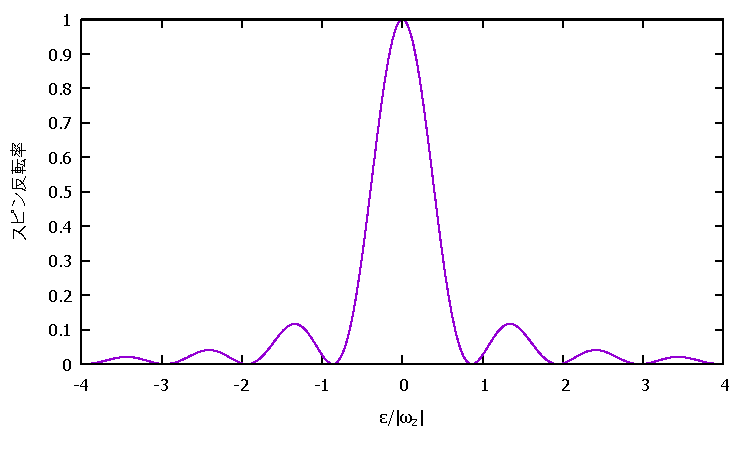
\includegraphics[width=10cm]{nonreso/nonreso_reversalrate.pdf}
\caption{スピン反転率}
\label{Nonreso_fig_reversalrate}
\end{center}
\end{figure}


\subsection{スピン干渉の原理}
ではいよいよ必ずしも共鳴条件を満たさない場合のスピン干渉の原理を見てゆこう。

\paragraph{舞台とあらすじ}
一様磁場中に、理想化されたRFスピンフリッパーふたつとシフタコイルひとつが置かれた状況を考える。系は7つの領域I,II,III,IV,V,VI,VIIからなり、全体に$z$方向一様磁場$B_z$がかけられ、それに加えて領域II,VIに$x$方向振動磁場$2B_r\cos\omega_s t$が、領域IVに$z$方向一様磁場$B$がかけられている。
\begin{figure}[h]
\centering
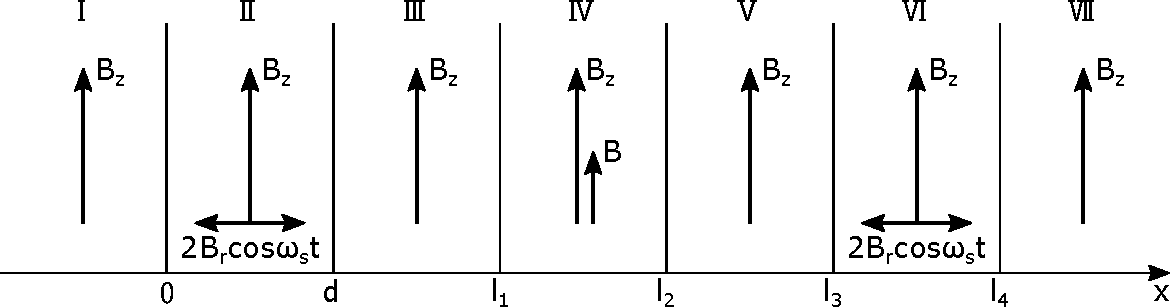
\includegraphics[height=3cm]{nonreso/resonance_setting2.pdf}
\end{figure}

これから述べるように、スピン上向きの中性子が領域Iから入射し、領域I$\sim$VIを通って領域VIIに抜けるとき、領域VIIにおいてスピン上向き中性子を観測する確率は
\begin{equation}
|\psi_\mathrm{VII}^+|^2=N_1(\epsilon)-N_2(\epsilon) \cos (\Omega -\Delta(\epsilon)) -N_3(\epsilon) \sin(\Omega-\Delta(\epsilon)) \label{Nonreso_interference}
\end{equation}
のように書ける。ここで$\Omega$はシフタコイル磁場によって生じた位相差、$\Delta(\epsilon)$は$\epsilon$に依存した定数位相である。

\paragraph{仮定と拝借}
今回は最初から中性子の入射エネルギーはポテンシャルに比べて十分大きいとし、全ての境界で反射は無視する。すると、前節での結果をそのまま拝借することができる。すなわち、領域I,II,IIIにおける波動関数はそれぞれ
\begin{align}
\psi_\mathrm{I}(x,t)&=\begin{pmatrix} 1\\0\end{pmatrix} \e^{i (k_0-\frac{\omega_z}{v})x}\e^{-i\omega_0t}\\
\psi_\mathrm{II}(x,t)&=\begin{pmatrix} \left(\sin^2 \frac{\theta}{2} \e^{i\frac{\omega_A}{v}x} +\cos^2 \frac{\theta}{2} \e^{-i\frac{\omega_A}{v}x} \right) \e^{i(k_0-\frac{\omega_s}{v}) x} \e^{-i\omega_0 t} \\ \sin\frac{\theta}{2}\cos\frac{\theta}{2} \left(\e^{-i\frac{\omega_A}{v}x}-\e^{i\frac{\omega_A}{v}x}\right) \e^{i(k_0-\frac{\omega_s}{v}) x} \e^{-i(\omega_0-\omega_s) t}\end{pmatrix}\\
\psi_\mathrm{III}(x,t)&=\begin{pmatrix} \left(\cos \frac{\omega_A}{v}d +i\frac{\epsilon}{\omega_A} \sin \frac{\omega_A}{v}d\right) \e^{-i\frac{\epsilon}{v} d} \e^{i(k_0-\frac{\omega_z}{v})x}\e^{-i\omega_0t} \\ -i \frac{\omega_r}{\omega_A} \sin \frac{\omega_A}{v}d  \, \e^{i\frac{\epsilon}{v}d} \e^{i(k_0-\frac{\omega_s}{v}+\frac{\omega_z}{v})x}\e^{-i(\omega_0-\omega_s)t} \end{pmatrix}
\end{align}
と書ける。ここで$\epsilon=\omega_s/2-\omega_z,\omega_A=\sqrt{\epsilon^2+\omega_r^2}$であり、$\omega_z=|\mu_n|B_z,\omega_r=|\mu_n|B_r$。$\omega_0$,$v$はそれぞれ中性子の入射エネルギー、速度であり、$k_0=\sqrt{2m\omega_0}$である。その他の記号は前節参照。

\paragraph{領域IV}
領域IVにおけるShr$\ddot{\mathrm{o}}$dinger方程式は
\begin{equation}
i\frac{\del \psi_\mathrm{IV}}{\del t}= \left[-\frac{1}{2m} \frac{\del^2}{\del x^2} +(\omega_z+\omega) \sigma_z\right] \psi_\mathrm{IV}
\end{equation}
ここで$\omega=|\mu_n|B$とした。領域IIIとIVの境界でエネルギーは変化しないので、領域IVにおけるスピン上下成分の波数$k^\pm_\mathrm{IV}$は
\begin{align}
k^+_\mathrm{IV}&=\sqrt{2m(\omega_0-(\omega_z+\omega))}\simeq k_0 -\frac{\omega_z}{v}-\frac{\omega}{v} \\
k^-_\mathrm{IV}&=\sqrt{2m(\omega_0-\omega_s+(\omega_z+\omega))}\simeq k_0 -\frac{\omega_s}{v}+\frac{\omega_z}{v}+\frac{\omega}{v}
\end{align}
となる。反射波を無視し、領域IIIとIVの境界($x=l_1$)で波動関数を接続すると
\begin{equation}
\psi_\mathrm{IV}=\begin{pmatrix} \left(\cos \frac{\omega_A}{v}d +i\frac{\epsilon}{\omega_A} \sin \frac{\omega_A}{v}d\right) \e^{-i\frac{\epsilon}{v} d} \e^{-i\frac{\omega}{v} (x-l_1)} \e^{i(k_0-\frac{\omega_z}{v})x}\e^{-i\omega_0t} \\ -i \frac{\omega_r}{\omega_A} \sin \frac{\omega_A}{v}d  \, \e^{i\frac{\epsilon}{v}d} \e^{i\frac{\omega}{v}(x-l_1)} \e^{i(k_0-\frac{\omega_s}{v}+\frac{\omega_z}{v})x}\e^{-i(\omega_0-\omega_s)t} \end{pmatrix}
\end{equation}
を得る。

\paragraph{領域V}
領域VにおけるShr$\ddot{\mathrm{o}}$dinger方程式は領域I,IIIと等しく、
\begin{equation}
i\frac{\del \psi_\mathrm{V}}{\del t}= \left[-\frac{1}{2m} \frac{\del^2}{\del x^2} +\omega_z \sigma_z\right] \psi_\mathrm{V}
\end{equation}
である。領域IVと同様にして、反射波を無視し、領域IVとVの境界($x=l_2$)で波動関数を接続すると
\begin{equation}
\psi_\mathrm{V}=\begin{pmatrix} \left(\cos \frac{\omega_A}{v}d +i\frac{\epsilon}{\omega_A} \sin \frac{\omega_A}{v}d\right) \e^{-i\frac{\epsilon}{v} d} \e^{-i\frac{\omega}{v} d'} \e^{i(k_0-\frac{\omega_z}{v})x}\e^{-i\omega_0t} \\ -i \frac{\omega_r}{\omega_A} \sin \frac{\omega_A}{v}d  \, \e^{i\frac{\epsilon}{v}d} \e^{i\frac{\omega}{v} d'} \e^{i(k_0-\frac{\omega_s}{v}+\frac{\omega_z}{v})x}\e^{-i(\omega_0-\omega_s)t} \end{pmatrix} \label{Nonreso_psi5}
\end{equation}
を得る。ここで$l_2-l_1=d'$を用いた。

\paragraph{領域VI}
領域VIにおける磁場を、領域IIと同じ$z$方向一様磁場と同位相の$x$方向振動磁場
\begin{equation}
\bm{B}_\mathrm{VI}=\hat{\bm{x}}(2B_r)\cos\omega_s t +\hat{\bm{z}}B_z
\end{equation}
とすると、$B_r \ll B_z$のとき
\begin{equation}
\bm{B}_\mathrm{VI} \simeq \hat{\bm{x}} B_r\cos \omega_s t+\hat{\bm{y}} B_r \sin \omega_s t+\hat{\bm{z}} B_z
\end{equation}
と近似でき、前節と同じ議論により領域VIにおける波動関数は次のように書ける:
\begin{equation}
\psi_\mathrm{VI}=\begin{pmatrix} \left(D^+\cos\frac{\theta}{2} \e^{-i\frac{\omega_A}{v} x}-D^-\sin\frac{\theta}{2} \e^{i\frac{\omega_A}{v}x} \right) \e^{i(k_0-\frac{\omega_s}{2v})x} \e^{-i\omega_0 t} \\ \left(D^+\sin\frac{\theta}{2}\e^{-i\frac{\omega_A}{v} x}+D^-\cos\frac{\theta}{2}\e^{i\frac{\omega_A}{v} x}\right) \e^{i(k_0-\frac{\omega_s}{2v})x} \e^{-i(\omega_0-\omega_s) t} \end{pmatrix}
\end{equation}
ここで入射エネルギーは十分大きいとして反射波を無視し、波数を
\begin{equation}
k^\pm_1 =\sqrt{2m\left(\omega_0-\frac{\omega_s}{2}\mp\omega_A\right)} \simeq k_0 -\frac{\omega_s}{2v} \mp\frac{\omega_A}{v}
\end{equation}
と近似した。また、$\cos \theta = -\epsilon/\omega_A,\sin\theta=\omega_r/\omega_A$であり、$D^\pm$は定数である。

\paragraph{領域VとVIの接続}簡単のため式(\ref{Nonreso_psi5})で
\begin{align}
\alpha^+ &= \left(\cos \frac{\omega_A}{v}d +i\frac{\epsilon}{\omega_A} \sin \frac{\omega_A}{v}d\right) \e^{-i\frac{\epsilon}{v} d} \e^{-i\frac{\omega}{v} d} \label{Nonreso_alpha+}\\
\alpha^-&=-i \frac{\omega_r}{\omega_A} \sin \frac{\omega_A}{v}d  \, \e^{i\frac{\epsilon}{v}d} \e^{i\frac{\omega}{v} d} \label{Nonreso_alpha-}
\end{align}
とおき、領域Vでの波動関数を
\begin{equation}
\psi_\mathrm{V} =\begin{pmatrix} \alpha^+ \e^{i(k_0-\frac{\omega_z}{v})x}\e^{-i\omega_0t}\\ \alpha^- \e^{i(k_0-\frac{\omega_s}{v}+\frac{\omega_z}{v})x}\e^{-i(\omega_0-\omega_s)t} \end{pmatrix}
\end{equation}
とかく。領域VとVIの境界($x=l_3$)における接続を考えて、次の2式を得る:
\begin{align}
&\left\{\begin{array}{l} \left(D^+ \cos\frac{\theta}{2} \e^{-i\frac{\omega_A}{v} l_3}-D^-\sin\frac{\theta}{2} \e^{i\frac{\omega_A}{v}l_3}\right) \e^{i(k_0-\frac{\omega_s}{2v})l_3} =\alpha^+ \e^{i(k_0-\frac{\omega_z}{v})l_3} \\ \left(D^+\sin\frac{\theta}{2}\e^{-i\frac{\omega_A}{v} l_3}+D^-\cos\frac{\theta}{2}\e^{i\frac{\omega_A}{v} l_3}\right) \e^{i(k_0-\frac{\omega_s}{2v})l_3} =\alpha^- \e^{i(k_0-\frac{\omega_s}{v}+\frac{\omega_z}{v})l_3}\end{array} \right. \notag \\
&\Rightarrow \left\{\begin{array}{l} D^+ \cos\frac{\theta}{2} \e^{-i\frac{\omega_A}{v} l_3}-D^-\sin\frac{\theta}{2} \e^{i\frac{\omega_A}{v}l_3} =\alpha^+ \e^{i\frac{\epsilon}{v}l_3} \\ D^+\sin\frac{\theta}{2}\e^{-i\frac{\omega_A}{v} l_3}+D^-\cos\frac{\theta}{2}\e^{i\frac{\omega_A}{v} l_3} =\alpha^- \e^{-i\frac{\epsilon}{v}l_3}\end{array} \right. \notag \\
&\Rightarrow \left\{\begin{array}{l} D^+ =\left(\alpha^+ \cos\frac{\theta}{2}\e^{i\frac{\epsilon}{v}l_3} +\alpha^- \sin\frac{\theta}{2}\e^{-i\frac{\epsilon}{v}l_3}\right) \e^{i\frac{\omega_A}{v} l_3} \\ D^-=\left(-\alpha^+ \sin\frac{\theta}{2} \e^{i\frac{\epsilon}{v}l_3} +\alpha^-\cos\frac{\theta}{2}\e^{-i\frac{\epsilon}{v}l_3} \right)\e^{-i\frac{\omega_A}{v} l_3} \end{array} \right.
\end{align}
したがって
\begin{equation}
\psi_\mathrm{VI} =\left( \begin{array}{l} \left[\alpha^+ \left(\cos^2\frac{\theta}{2}\e^{-i\frac{\omega_A}{v}(x-l_3)} +\sin^2\frac{\theta}{2}\e^{i\frac{\omega_A}{v}(x-l_3)} \right)\e^{i\frac{\epsilon}{v}l_3} \right. \\ \hspace{2cm}\left. +\alpha^- \sin\frac{\theta}{2}\cos\frac{\theta}{2} \left(\e^{-i\frac{\omega_A}{v}(x-l_3)}-\e^{i\frac{\omega_A}{v}(x-l_3)}\right)\e^{-i\frac{\epsilon}{v}l_3}\right]\e^{i(k_0-\frac{\omega_s}{2v})x}\e^{-\omega_0t} \\ \left[\alpha^+ \sin\frac{\theta}{2}\cos\frac{\theta}{2} \left(\e^{-i\frac{\omega_A}{v}(x-l_3)}-\e^{i\frac{\omega_A}{v}(x-l_3)}\right)\e^{i\frac{\epsilon}{v}l_3} \right. \\ \hspace{2cm} \left. +\alpha^- \left(\sin^2\frac{\theta}{2}\e^{-i\frac{\omega_A}{v}(x-l_3)} +\cos^2\frac{\theta}{2}\e^{i\frac{\omega_A}{v}(x-l_3)} \right) \e^{-i\frac{\epsilon}{v}l_3}\right] \e^{i(k_0-\frac{\omega_s}{2v})x} \e^{-i(\omega_0-\omega_s) t} \end{array}\right)
\end{equation}
となる。

\paragraph{領域VII}
領域VにおけるShr$\ddot{\mathrm{o}}$dinger方程式は領域I,III,Vと同じく
\begin{equation}
i\frac{\del \psi_\mathrm{VII}}{\del t}= \left[-\frac{1}{2m} \frac{\del^2}{\del x^2} +\omega_z \sigma_z\right] \psi_\mathrm{VII}
\end{equation}
であり、領域VIとVIIの境界($x=l_4$)で波動関数を接続すると次式を得る:
\begin{align}
\psi_\mathrm{VII} &=\left( \begin{array}{l} \left[\alpha^+ \left(\cos^2\frac{\theta}{2}\e^{-i\frac{\omega_A}{v}(l_4-l_3)} +\sin^2\frac{\theta}{2}\e^{i\frac{\omega_A}{v}(l_4-l_3)} \right)\e^{i\frac{\epsilon}{v}l_3} \right. \\ \hspace{1cm}\left. +\alpha^- \sin\frac{\theta}{2}\cos\frac{\theta}{2} \left(\e^{-i\frac{\omega_A}{v}(l_4-l_3)}-\e^{i\frac{\omega_A}{v}(l_4-l_3)}\right)\e^{-i\frac{\epsilon}{v}l_3}\right]\e^{i(k_0-\frac{\omega_s}{2v})l_4} \e^{i(k_0-\frac{\omega_z}{v})(x-l_4)} \e^{-\omega_0t} \\ \left[\alpha^+ \sin\frac{\theta}{2}\cos\frac{\theta}{2} \left(\e^{-i\frac{\omega_A}{v}(l_4-l_3)}-\e^{i\frac{\omega_A}{v}(l_4-l_3)}\right)\e^{i\frac{\epsilon}{v}l_3} \right. \\ \hspace{1cm} \left. +\alpha^- \left(\sin^2\frac{\theta}{2}\e^{-i\frac{\omega_A}{v}(l_4-l_3)} +\cos^2\frac{\theta}{2}\e^{i\frac{\omega_A}{v}(l_4-l_3)} \right) \e^{-i\frac{\epsilon}{v}l_3}\right] \e^{i(k_0-\frac{\omega_s}{2v})l_4} \e^{i(k_0-\frac{\omega_s}{v}+\frac{\omega_z}{v})(x-l_4)} \e^{-i(\omega_0-\omega_s) t} \end{array}\right) \notag \\
&=\left( \begin{array}{l} \left[\alpha^+ \left(\cos^2\frac{\theta}{2}\e^{-i\frac{\omega_A}{v}d} +\sin^2\frac{\theta}{2}\e^{i\frac{\omega_A}{v}d} \right)\e^{i\frac{\epsilon}{v}l_3} \right. \\ \hspace{2cm}\left. +\alpha^- \sin\frac{\theta}{2}\cos\frac{\theta}{2} \left(\e^{-i\frac{\omega_A}{v}d}-\e^{i\frac{\omega_A}{v}d}\right)\e^{-i\frac{\epsilon}{v}l_3}\right]\e^{-i\frac{\epsilon}{v}l_4}\e^{i(k_0-\frac{\omega_z}{v})x} \e^{-\omega_0t} \\ \left[\alpha^+ \sin\frac{\theta}{2}\cos\frac{\theta}{2} \left(\e^{-i\frac{\omega_A}{v}d}-\e^{i\frac{\omega_A}{v}d}\right)\e^{i\frac{\epsilon}{v}l_3} \right. \\ \hspace{2cm} \left. +\alpha^- \left(\sin^2\frac{\theta}{2}\e^{-i\frac{\omega_A}{v}d} +\cos^2\frac{\theta}{2}\e^{i\frac{\omega_A}{v}d} \right) \e^{-i\frac{\epsilon}{v}l_3}\right] \e^{i\frac{\epsilon}{v}l_4} \e^{i(k_0-\frac{\omega_s}{v}+\frac{\omega_z}{v})x} \e^{-i(\omega_0-\omega_s) t} \end{array}\right)
\end{align}
ここで$l_4-l_3=d$を用いた。さらに$\cos\theta=-\epsilon/\omega_A,\sin\theta=\omega_r/\omega_A$より
\begin{align}
&\cos^2 \frac{\theta}{2} \e^{-i\frac{\omega_A}{v}d} +\sin^2 \frac{\theta}{2} \e^{i\frac{\omega_A}{v}d} =\cos \frac{\omega_A}{v}d +i\frac{\epsilon}{\omega_A} \sin \frac{\omega_A}{v}d \\
&\sin^2 \frac{\theta}{2} \e^{-i\frac{\omega_A}{v}d} +\cos^2 \frac{\theta}{2} \e^{i\frac{\omega_A}{v}d} =\left(\cos^2 \frac{\theta}{2} \e^{-i\frac{\omega_A}{v}d} +\sin^2 \frac{\theta}{2} \e^{i\frac{\omega_A}{v}d}\right)^\dagger=\cos \frac{\omega_A}{v}d -i\frac{\epsilon}{\omega_A} \sin \frac{\omega_A}{v}d \\
&\sin\frac{\theta}{2}\cos\frac{\theta}{2} \left(\e^{-i\frac{\omega_A}{v}d}-\e^{i\frac{\omega_A}{v}d}\right) = -i \frac{\omega_r}{\omega_A} \sin \frac{\omega_A}{v}d
\end{align}
を用い、(\ref{Nonreso_alpha+}),(\ref{Nonreso_alpha-})の$\alpha^\pm$を代入して
\begin{align}
\psi_\mathrm{VII} &= \left( \begin{array}{l} \left[\left(\cos \frac{\omega_A}{v}d +i\frac{\epsilon}{\omega_A} \sin \frac{\omega_A}{v}d\right)^2\e^{i\frac{\epsilon}{v}(l_3-d)}\e^{-i\frac{\omega}{v}d'} \right. \\ \hspace{2cm}\left. +\left(-i \frac{\omega_r}{\omega_A} \sin \frac{\omega_A}{v}d\right)^2\e^{-i\frac{\epsilon}{v}(l_3-d)}\e^{i\frac{\omega}{v}d'} \right]\e^{-i\frac{\epsilon}{v}l_4}\e^{i(k_0-\frac{\omega_z}{v})x} \e^{-\omega_0t} \\ \left[\left(\cos \frac{\omega_A}{v}d +i\frac{\epsilon}{\omega_A} \sin \frac{\omega_A}{v}d\right) \left(-i \frac{\omega_r}{\omega_A} \sin \frac{\omega_A}{v}d\right) \e^{i\frac{\epsilon}{v}(l_3-d)}\e^{-i\frac{\omega}{v}d'} \right. \\ \hspace{1cm} \left. +\left(-i \frac{\omega_r}{\omega_A} \sin \frac{\omega_A}{v}d\right) \left(\cos \frac{\omega_A}{v}d -i\frac{\epsilon}{\omega_A} \sin \frac{\omega_A}{v}d\right) \e^{-i\frac{\epsilon}{v}(l_3-d)}\e^{i\frac{\omega}{v}d'} \right] \e^{i\frac{\epsilon}{v}l_4} \e^{i(k_0-\frac{\omega_s}{v}+\frac{\omega_z}{v})x} \e^{-i(\omega_0-\omega_s) t} \end{array}\right) \notag \\
&=\left( \begin{array}{l} \left[\left(\cos \frac{\omega_A}{v}d +i\frac{\epsilon}{\omega_A} \sin \frac{\omega_A}{v}d\right)^2\e^{i\frac{\epsilon}{v}L'}\e^{-i\frac{\omega}{v}d'} \right. \\ \hspace{2cm}\left. +\left(-i \frac{\omega_r}{\omega_A} \sin \frac{\omega_A}{v}d\right)^2\e^{-i\frac{\epsilon}{v}L'}\e^{i\frac{\omega}{v}d'} \right]\e^{-i\frac{\epsilon}{v}L}\e^{i(k_0-\frac{\omega_z}{v})x} \e^{-\omega_0t} \\ \left(-i \frac{\omega_r}{\omega_A} \sin \frac{\omega_A}{v}d\right) \left[\left(\cos \frac{\omega_A}{v}d +i\frac{\epsilon}{\omega_A} \sin \frac{\omega_A}{v}d\right) \e^{i\frac{\epsilon}{v}L'}\e^{-i\frac{\omega}{v}d'} \right. \\ \hspace{2cm} \left. +\left(\cos \frac{\omega_A}{v}d -i\frac{\epsilon}{\omega_A} \sin \frac{\omega_A}{v}d\right) \e^{-i\frac{\epsilon}{v}L'}\e^{i\frac{\omega}{v}d'} \right] \e^{i\frac{\epsilon}{v}L} \e^{i(k_0-\frac{\omega_s}{v}+\frac{\omega_z}{v})x} \e^{-i(\omega_0-\omega_s) t} \end{array}\right)
\end{align}
となる。ここで$l_3-d=L',l_4=L$とした。
%\end{comment}


\paragraph{結末}
以上のようにして、領域Iで
\begin{equation}
\psi_\mathrm{I}(x,t)=\begin{pmatrix} 1\\0\end{pmatrix} \e^{i (k_0-\frac{\omega_z}{v})x}\e^{-i\omega_0t}
\end{equation}
と表された入射中性子は領域II$\sim$VIを通って領域VIIで
\begin{equation}
\psi_\mathrm{VII}(x,t) =\left( \begin{array}{l} \left[\left(\cos \frac{\omega_A}{v}d +i\frac{\epsilon}{\omega_A} \sin \frac{\omega_A}{v}d\right)^2\e^{i\frac{\epsilon}{v}L'}\e^{-i\frac{\omega}{v}d'} \right. \\ \hspace{2cm}\left. +\left(-i \frac{\omega_r}{\omega_A} \sin \frac{\omega_A}{v}d\right)^2\e^{-i\frac{\epsilon}{v}L'}\e^{i\frac{\omega}{v}d'} \right]\e^{-i\frac{\epsilon}{v}L}\e^{i(k_0-\frac{\omega_z}{v})x} \e^{-\omega_0t} \\ \left(-i \frac{\omega_r}{\omega_A} \sin \frac{\omega_A}{v}d\right) \left[\left(\cos \frac{\omega_A}{v}d +i\frac{\epsilon}{\omega_A} \sin \frac{\omega_A}{v}d\right) \e^{i\frac{\epsilon}{v}L'}\e^{-i\frac{\omega}{v}d'} \right. \\ \hspace{2cm} \left. +\left(\cos \frac{\omega_A}{v}d -i\frac{\epsilon}{\omega_A} \sin \frac{\omega_A}{v}d\right) \e^{-i\frac{\epsilon}{v}L'}\e^{i\frac{\omega}{v}d'} \right] \e^{i\frac{\epsilon}{v}L} \e^{i(k_0-\frac{\omega_s}{v}+\frac{\omega_z}{v})x} \e^{-i(\omega_0-\omega_s) t} \end{array}\right)
\end{equation}
という状態をとることがわかった。したがって、領域VIIでスピン上向き中性子を観測する確率は
\begin{align}
|\psi_\mathrm{VII}^+|^2&=\Biggl| \left(\cos \frac{\omega_A}{v}d +i\frac{\epsilon}{\omega_A} \sin \frac{\omega_A}{v}d\right)^2\e^{i\frac{\epsilon}{v}L'}\e^{-i\frac{\omega}{v}d'} +\left(-i \frac{\omega_r}{\omega_A} \sin \frac{\omega_A}{v}d\right)^2\e^{-i\frac{\epsilon}{v}L'}\e^{i\frac{\omega}{v}d'} \Biggr|^2 \notag \\
&=\left[\left(\cos \frac{\omega_A}{v}d +i\frac{\epsilon}{\omega_A} \sin \frac{\omega_A}{v}d\right)^2\e^{i\frac{\epsilon}{v}L'}\e^{-i\frac{\omega}{v}d'} +\left(-i \frac{\omega_r}{\omega_A} \sin \frac{\omega_A}{v}d\right)^2\e^{-i\frac{\epsilon}{v}L'}\e^{i\frac{\omega}{v}d'}\right] \notag\\
&\hspace{2cm} \times \left[\left(\cos \frac{\omega_A}{v}d -i\frac{\epsilon}{\omega_A} \sin \frac{\omega_A}{v}d\right)^2\e^{-i\frac{\epsilon}{v}L'}\e^{i\frac{\omega}{v}d'} +\left(i \frac{\omega_r}{\omega_A} \sin \frac{\omega_A}{v}d\right)^2\e^{i\frac{\epsilon}{v}L'}\e^{-i\frac{\omega}{v}d'}\right] \notag \\
&=\left(\cos^2 \frac{\omega_A}{v}d +\left(\frac{\epsilon}{\omega_A}\right)^2 \sin^2 \frac{\omega_A}{v}d\right)^2+\left(\frac{\omega_r}{\omega_A}\right)^4 \sin^4 \frac{\omega_A}{v}d \notag \\
&\hspace{1cm}  -2\left(\frac{\omega_r}{\omega_A}\right)^2\sin^2\frac{\omega_A}{v}d \left[\left(\cos^2 \frac{\omega_A}{v}d -\left(\frac{\epsilon}{\omega_A}\right)^2 \sin^2 \frac{\omega_A}{v}d\right) \cos \left(\frac{2}{v}(\omega d'-\epsilon L')\right) \right. \notag \\
&\hspace{6.3cm} \left.+2 \frac{\epsilon}{\omega_A} \sin \frac{\omega_A}{v}d \cos \frac{\omega_A}{v}d \sin \left(\frac{2}{v}(\omega d'-\epsilon L')\right)\right]
\end{align}
となる。
\begin{align}
&N_1 = \left(\cos^2 \frac{\omega_A}{v}d +\left(\frac{\epsilon}{\omega_A}\right)^2 \sin^2 \frac{\omega_A}{v}d\right)^2+\left(\frac{\omega_r}{\omega_A}\right)^4 \sin^4 \frac{\omega_A}{v}d \\
&N_2 = 2\left(\frac{\omega_r}{\omega_A}\right)^2\sin^2\frac{\omega_A}{v}d \left(\cos^2 \frac{\omega_A}{v}d -\left(\frac{\epsilon}{\omega_A}\right)^2 \sin^2 \frac{\omega_A}{v}d\right) \\
&N_3 = 4\frac{\epsilon}{\omega_A} \left(\frac{\omega_r}{\omega_A}\right)^2\sin^3\frac{\omega_A}{v}d \cos \frac{\omega_A}{v}d
\end{align}
とおけばこれを
\begin{equation}
|\psi_\mathrm{VII}^+|^2 =N_1 -N_2 \cos \left(\frac{2}{v}(\omega d'-\epsilon L')\right)-N_3 \sin  \left(\frac{2}{v}(\omega d'-\epsilon L')\right) \label{Nonreso_interference2}
\end{equation}
と書くことができる。

いま$\omega_rd/v=\pi/4$,$\epsilon/|\omega_z|=0,0.3,0.5,1.0$のときに$\omega d'/v$と$|\psi_\mathrm{VII}|^2$の関係を図示すると図\ref{Nonreso_fig_interference}のようになる。ただし$L'/d=10$とした。このように理論が予想するところによると、シフタコイルの磁場を変えながら領域VIIでスピン上向き中性子の数を計測すると波打つ干渉のパターンが見られるが、その振幅や位相、振動中心の位置は共鳴からのずれによって異なる。

\begin{figure}[h]
\centering
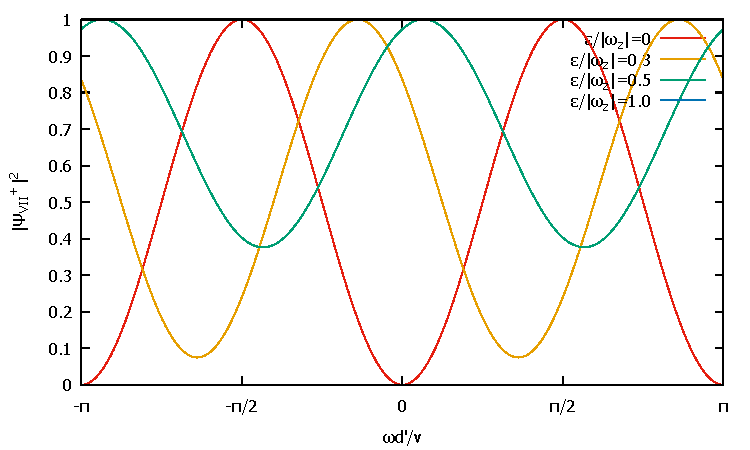
\includegraphics[width=10cm]{nonreso/nonreso_interference.pdf}
\caption{干渉パターン {\footnotesize ($\epsilon/|\omega_z|=1.0$は上に張り付いている)}}
\label{Nonreso_fig_interference}
\vspace{-1cm}
\end{figure}



\renewcommand{\arraystretch}{1}


